
\section{Q2}
\label{part2}
\begin{enumerate}

\item 2.1 Using the pages from Q1 (A4), download all TimeMaps (including TimeMaps with 404 responses, i.e. empty or null TimeMaps) 
\subitem - Upload all the TimeMaps to github

\item 2.2 Build a CDF for number of mementos for each original URI (i.e., x-axis = number of mementos, y-axis = percentage of links)

\subitem See: \url{http://timetravel.mementoweb.org/guide/api/}



\end{enumerate}

\subsection{Solution}
\begin{enumerate}

\item I wrote a python program to fetch the timemaps. The aggregrator that I used is \url{http://labs.mementoweb.org/timemap/json/}
\item Following is the graph showing CDF for number of mementos for each original URI:

\begin{figure}[ht]    
    \begin{center}
        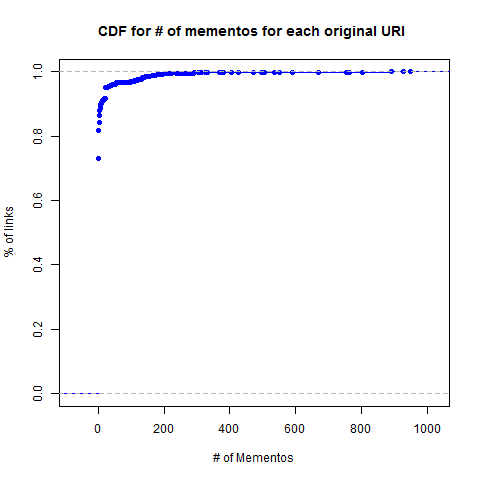
\includegraphics[scale=0.60]{graphs/2_mementoCount.png}
        \caption{Examples}        
    \end{center}
\end{figure}


\newpage
\subsection{Code Listing}
\subsubsection{Python program to fetch the timemaps for the URIs from Q1 on which boilerpipe is successful}
\lstinputlisting[language=Python,breaklines = true,frame=single, label=lst:q1-1,captionpos=b,numbers=left,showspaces=false,showstringspaces=false,basicstyle=\footnotesize]{src/2.1fetchTimemaps.py}
\newpage

\subsubsection{Python program to count the mementos for each Timemap}
\lstinputlisting[language=Python,breaklines = true,frame=single,label=lst:q1-1,captionpos=b,numbers=left,showspaces=false,showstringspaces=false,basicstyle=\footnotesize]{src/2.2countMementos.py}
\newpage

\subsubsection{R code to plot CDF}
\lstinputlisting[language=Python,breaklines = true,frame=single, label=lst:q1-1,captionpos=b,numbers=left,showspaces=false,showstringspaces=false,basicstyle=\footnotesize]{src/2.r}
\newpage

\newpage


\end{enumerate}
